%**************************************************************************************
% License:
% CC BY-NC-SA 4.0 (http://creativecommons.org/licenses/by-nc-sa/4.0/)
%**************************************************************************************

\documentclass[notes]{beamer}

\mode<presentation> {

\usetheme{Madrid}

% Burnt orange
\definecolor{burntorange}{rgb}{0.8, 0.33, 0.0}
\colorlet{beamer@blendedblue}{burntorange}
% Pale yellow
\definecolor{paleyellow}{rgb}{1.0, 1.0, 0.953}
\setbeamercolor{background canvas}{bg=paleyellow}
% Secondary and tertiary palette
\setbeamercolor*{palette secondary}{use=structure,fg=white,bg=burntorange!80!black}
\setbeamercolor*{palette tertiary}{use=structure,fg=white,bg=burntorange!60!black}

% To remove the footer line in all slides uncomment this line
%\setbeamertemplate{footline}
% To replace the footer line in all slides with a simple slide count uncomment this line
%\setbeamertemplate{footline}[page number]

% To remove the navigation symbols from the bottom of all slides uncomment this line
%\setbeamertemplate{navigation symbols}{}
}

\usepackage{amsmath}
\DeclareMathOperator*{\argmin}{arg\,min}
\DeclareMathOperator*{\argmax}{arg\,max}
\usepackage{bm}
\usepackage{booktabs} % Allows the use of \toprule, \midrule and \bottomrule in tables
\usepackage{breqn}
\usepackage{cleveref}
\usepackage{graphicx} % for figures
\usepackage[labelsep=space,tableposition=top]{caption}
\renewcommand{\figurename}{Fig.} 
\usepackage{caption,subcaption}% http://ctan.org/pkg/{caption,subcaption}
\usepackage{xcolor}

% To print 2 slides on a page
%\usepackage{handoutWithNotes}
%\pgfpagesuselayout{2 on 1}[border shrink=2mm]

%----------------------------------------------------------------------------------------
%	TITLE PAGE
%----------------------------------------------------------------------------------------
% The short title appears at the bottom of every slide, the full title is only on the title page
\title[Neural Networks \& Function Approximation]{Neural Networks and Function Approximation} 
\author{Krishna Kumar} % name
\institute[UT Austin] % institution 
{
University of Texas at Austin \\
\medskip
\textit{
  \url{krishnak@utexas.edu}} % Your email address
}
\date{} % Date, can be changed to a custom date

\begin{document}

\begin{frame}
\titlepage % title page as the first slide
\end{frame}

\begin{frame}
 % Table of contents slide, comment this block out to remove it
 \frametitle{Overview}
 % Throughout your presentation, if you choose to use \section{} and \subsection{} 
 % commands, these %will automatically be printed on this slide as an overview 
 \tableofcontents
\end{frame}

%----------------------------------------------------------------------------------------
% slides
%----------------------------------------------------------------------------------------

\section{Introduction and Motivation}

%------------------------------------------------
\begin{frame}
\frametitle{The 1D Poisson Equation: Our Benchmark Problem}

Consider the one-dimensional Poisson equation on $[0, 1]$:

\mode<beamer>{
\begin{equation*}
-\frac{d^2u}{dx^2} = f(x), \quad x \in [0, 1]
\end{equation*}

with boundary conditions:
\begin{equation*}
u(0) = 0, \quad u(1) = 0
\end{equation*}

For $f(x) = \pi^2 \sin(\pi x)$, the analytical solution is:
\begin{equation*}
u(x) = \sin(\pi x)
\end{equation*}
}
\mode<handout>{
\vspace{3cm}
}

\begin{figure}[ht]
	\centering
	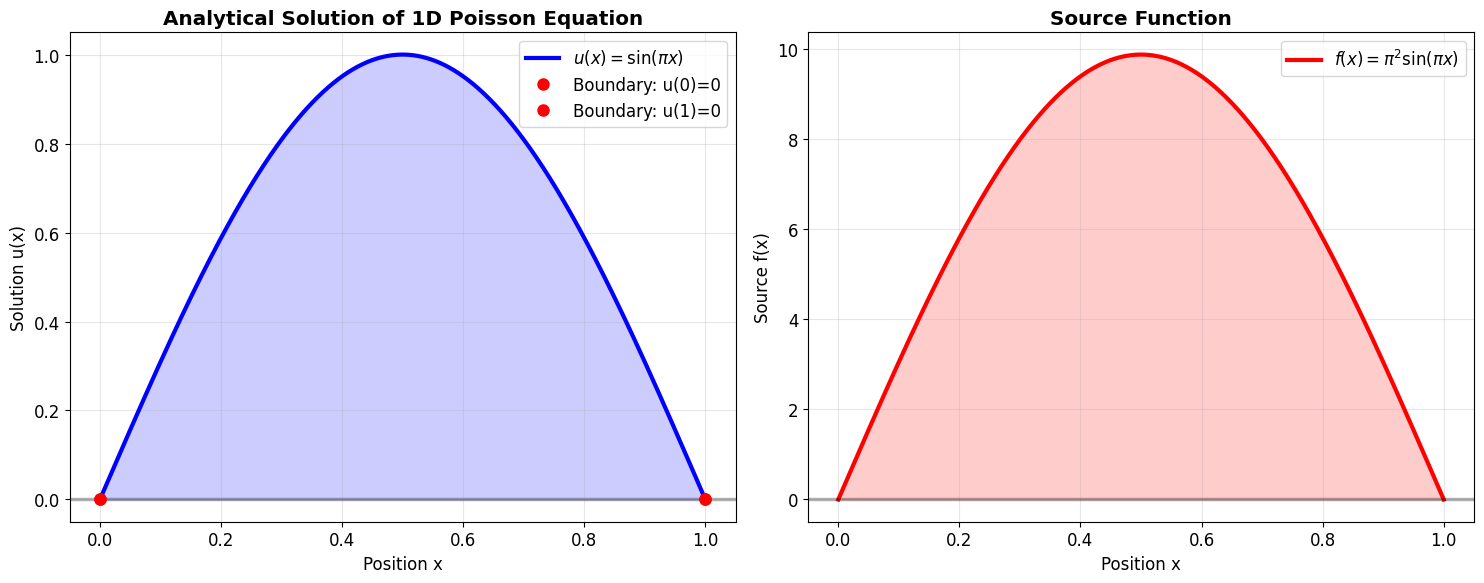
\includegraphics[width=0.8\textwidth]{figs/poisson-analytical-solution.png}
	\caption*{Analytical solution and source function}
\end{figure}

\end{frame}

%------------------------------------------------
\begin{frame}
\frametitle{The Function Approximation Challenge}

\textbf{Key Question:} Can we learn to approximate $u(x) = \sin(\pi x)$ from sparse data?

\begin{figure}[ht]
	\centering
	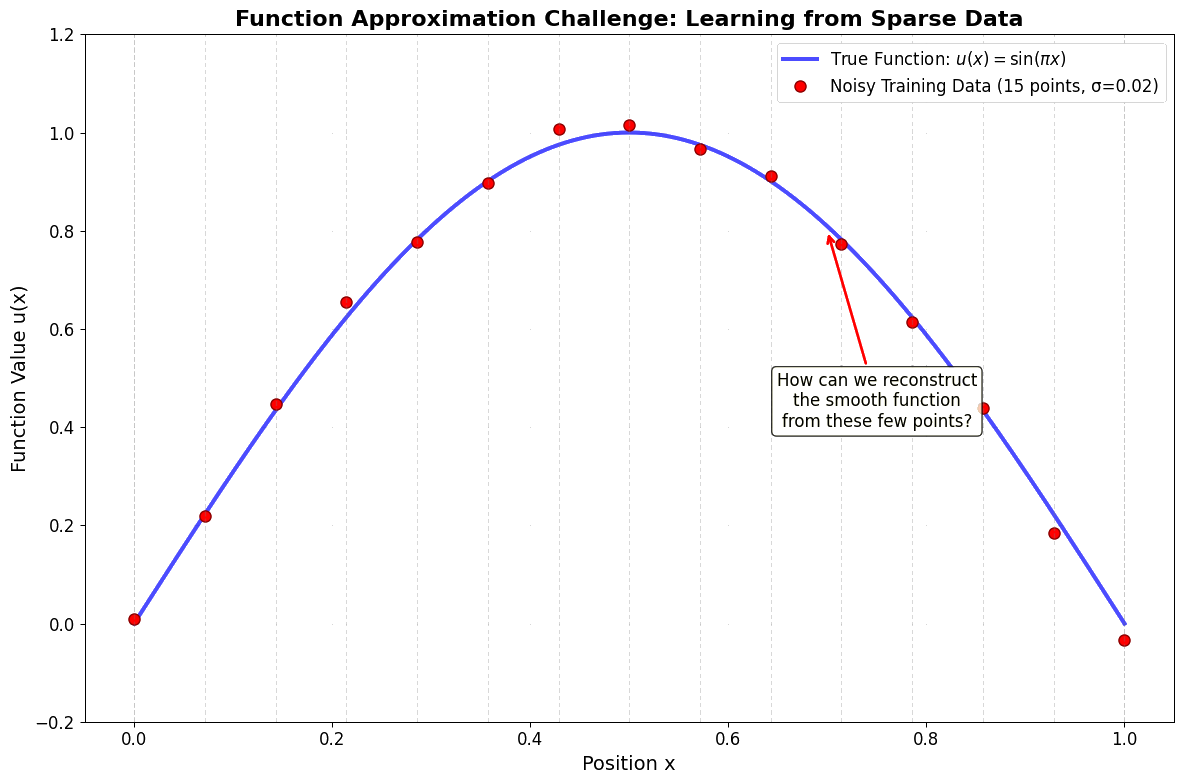
\includegraphics[width=0.9\textwidth]{figs/sparse-data-challenge.png}
	\caption*{Learning from 15 noisy training points}
\end{figure}

\textbf{Challenge:} Reconstruct a smooth, continuous function from limited observations.

\end{frame}

%------------------------------------------------
\begin{frame}
\frametitle{Traditional vs Neural Network Approaches}

\textbf{Traditional Methods (Finite Difference):}
\begin{itemize}
\item Discretize domain into grid points
\item Solve for values at specific locations
\item Result: Discrete representation
\end{itemize}

\mode<beamer>{
Finite difference approximation:
\begin{equation*}
\frac{d^2u}{dx^2} \approx \frac{u_{i+1} - 2u_i + u_{i-1}}{h^2}
\end{equation*}
}
\mode<handout>{
\vspace{1.5cm}
}

\textbf{Neural Network Approach:}
\begin{itemize}
\item Learn continuous function $u_{NN}(x; \theta)$
\item Approximate solution over entire domain
\item Parameters $\theta$ trained from sparse data
\end{itemize}

\end{frame}

%------------------------------------------------
\begin{frame}
\frametitle{Finite Difference vs Neural Networks}

\begin{figure}[ht]
	\centering
	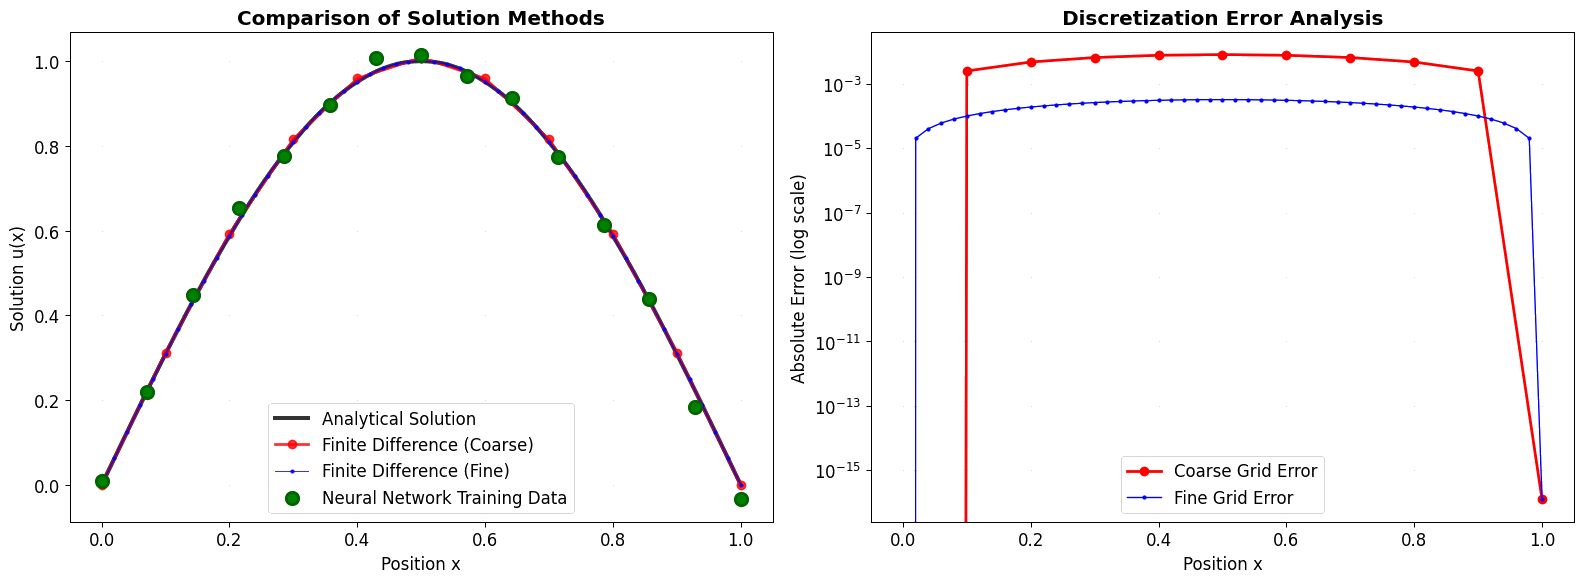
\includegraphics[width=0.9\textwidth]{figs/fd-poisson.png}
	\caption*{Comparison of solution methods and discretization errors}
\end{figure}

\textbf{Key Insight:} Neural networks learn continuous functions, not just discrete values.

\end{frame}

%------------------------------------------------
\section{Neural Network Fundamentals}

%------------------------------------------------
\begin{frame}
\frametitle{The Perceptron: Basic Building Block}

A perceptron computes:
\mode<beamer>{
\begin{align*}
z &= \mathbf{w}^T\mathbf{x} + b = \sum_{i=1}^n w_i x_i + b \\
\hat{y} &= g(z)
\end{align*}

where $g$ is the activation function.
}
\mode<handout>{
\vspace{2cm}
}

\begin{figure}[ht]
	\centering
	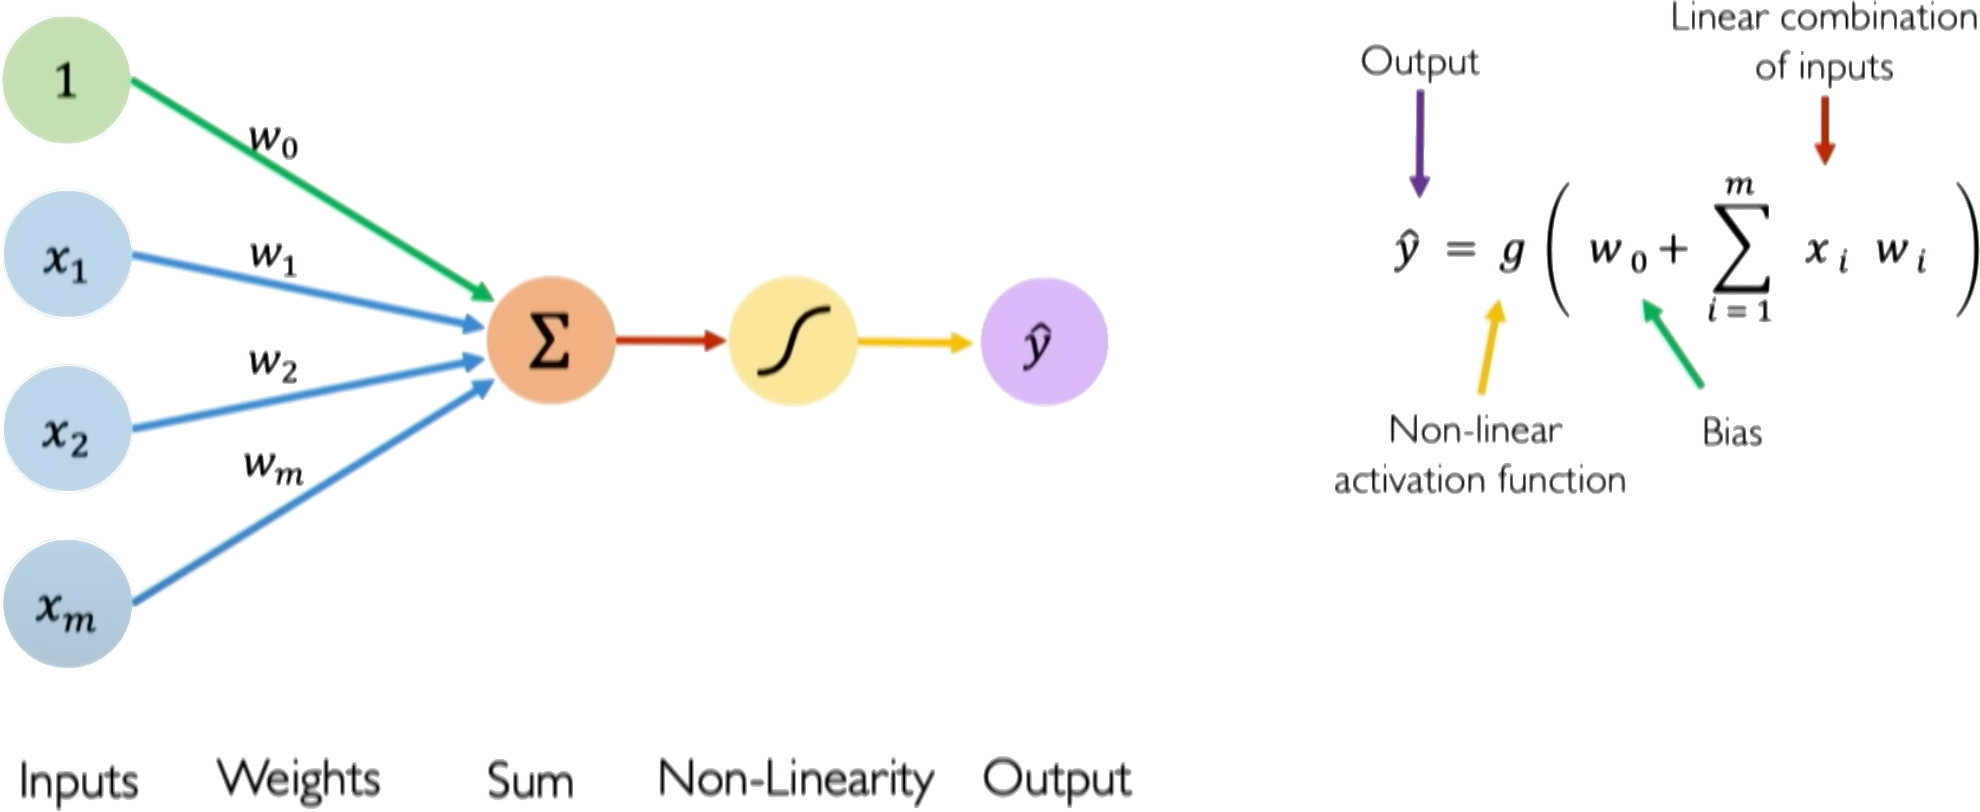
\includegraphics[width=0.7\textwidth]{figs/perceptron.png}
	\caption*{Perceptron architecture}
\end{figure}

\textbf{Key components:} Input vector, weights, bias, activation function, output.

\end{frame}

%------------------------------------------------
\begin{frame}
\frametitle{The Critical Role of Nonlinearity}

\textbf{Without activation functions:} Multiple linear layers collapse to single linear transformation.

\mode<beamer>{
Consider two linear layers:
\begin{align*}
h_1 &= W_1 x + b_1 \\
h_2 &= W_2 h_1 + b_2 = W_2(W_1 x + b_1) + b_2 \\
&= (W_2 W_1) x + (W_2 b_1 + b_2)
\end{align*}

This is equivalent to: $h_2 = W_{eq} x + b_{eq}$ (still linear!)
}
\mode<handout>{
\vspace{3cm}
}

\textbf{Problem:} Linear networks can only learn $y = mx + b$, but $\sin(\pi x)$ is curved!

\end{frame}

%------------------------------------------------
\begin{frame}
\frametitle{Demonstrating Linear Network Failure}

\begin{figure}[ht]
	\centering
	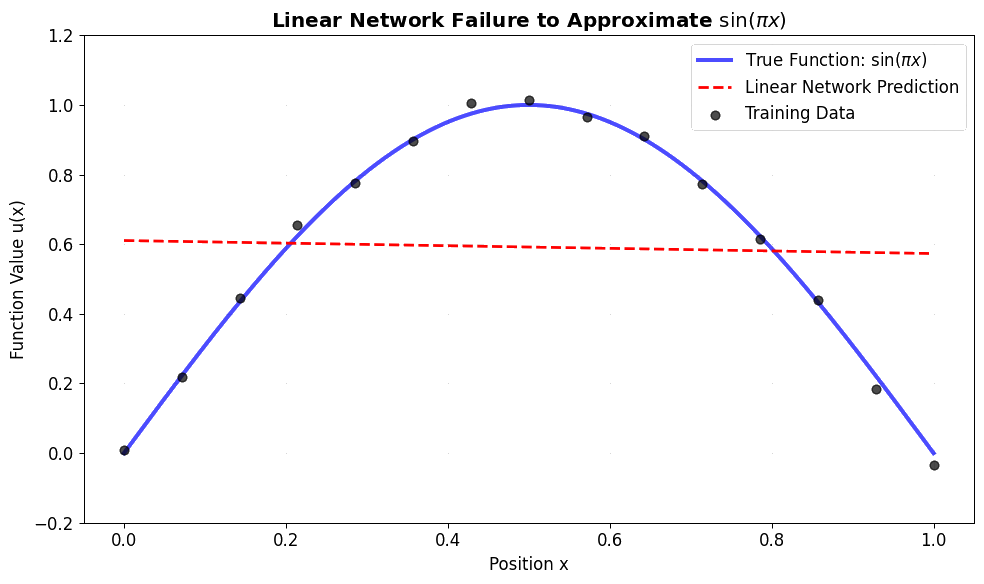
\includegraphics[width=0.9\textwidth]{figs/linear-network-failure.png}
	\caption*{Linear network cannot approximate $\sin(\pi x)$}
\end{figure}

\textbf{Conclusion:} Nonlinearity is essential for complex function approximation.

\end{frame}

%------------------------------------------------
\begin{frame}
\frametitle{Common Activation Functions}

\mode<beamer>{
\textbf{Sigmoid:} $\sigma(x) = \frac{1}{1 + e^{-x}}$ (squashes to (0,1))

\textbf{Tanh:} $\tanh(x) = \frac{e^x - e^{-x}}{e^x + e^{-x}}$ (squashes to (-1,1))

\textbf{ReLU:} $f(x) = \max(0, x)$ (efficient, prevents vanishing gradients)

\textbf{Leaky ReLU:} $f(x) = \max(\alpha x, x)$ (prevents dead neurons)
}
\mode<handout>{
\vspace{4cm}
}

\begin{figure}[ht]
	\centering
	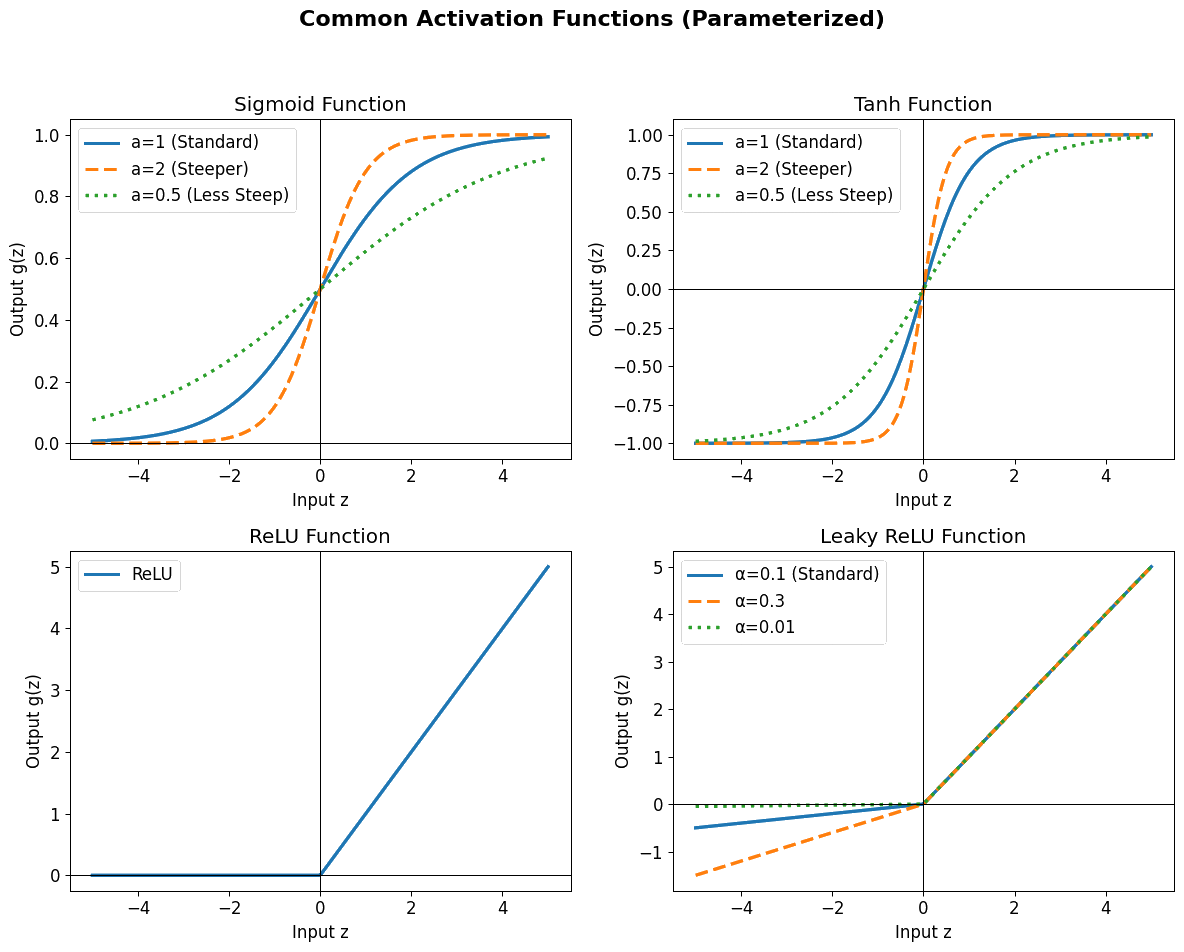
\includegraphics[width=0.8\textwidth]{figs/activation-functions.png}
	\caption*{Common activation functions}
\end{figure}

\end{frame}

%------------------------------------------------
\section{Universal Approximation Theorem}

%------------------------------------------------
\begin{frame}
\frametitle{Universal Approximation Theorem}

\textbf{Theorem (Cybenko, 1989):} A single hidden layer network with sufficient neurons can approximate any continuous function to arbitrary accuracy.

\mode<beamer>{
\begin{equation*}
F(x) = \sum_{i=1}^{N} w_i \sigma(v_i x + b_i) + w_0
\end{equation*}

\textbf{Mathematical statement:} For any continuous $f: [0,1] \to \mathbb{R}$ and $\epsilon > 0$, there exists $N$ and parameters such that $|F(x) - f(x)| < \epsilon$ for all $x \in [0,1]$.
}
\mode<handout>{
\vspace{3cm}
}

\textbf{Key Questions:}
\begin{itemize}
\item How many neurons $N$ do we need?
\item Is this practical?
\item Can we verify experimentally?
\end{itemize}

\end{frame}

%------------------------------------------------
\begin{frame}
\frametitle{Single Hidden Layer Architecture}

For 1D input $x$, a single-layer network with $N_h$ hidden neurons:

\mode<beamer>{
\begin{align*}
\mathbf{z}^{(1)} &= W^{(1)}x + \mathbf{b}^{(1)} \quad \text{(pre-activation)} \\
\mathbf{h} &= g(\mathbf{z}^{(1)}) \quad \text{(hidden layer output)} \\
z^{(2)} &= W^{(2)}\mathbf{h} + b^{(2)} \quad \text{(output layer)} \\
\hat{y} &= z^{(2)} \quad \text{(final prediction)}
\end{align*}
}
\mode<handout>{
\vspace{3cm}
}

\begin{figure}[ht]
	\centering
	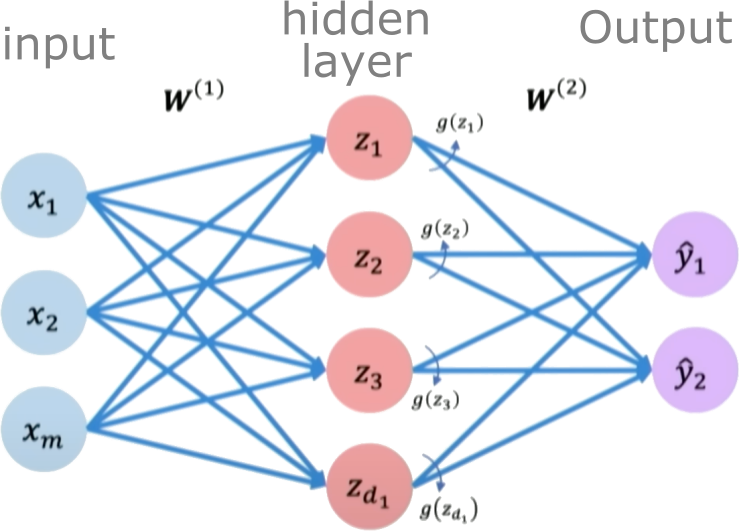
\includegraphics[width=0.7\textwidth]{figs/single-layer-nn2.png}
	\caption*{Single hidden layer neural network}
\end{figure}

\end{frame}

%------------------------------------------------
\section{Training Neural Networks}

%------------------------------------------------
\begin{frame}
\frametitle{Training Process}

\textbf{Goal:} Find optimal parameters $\theta^*$ that minimize loss function.

\mode<beamer>{
Loss function (MSE):
\begin{equation*}
\mathcal{L}(\theta) = \frac{1}{N} \sum_{i=1}^N \left(u_{NN}(x_i; \theta) - u_i\right)^2
\end{equation*}

Optimization problem:
\begin{equation*}
\theta^* = \argmin_{\theta} \mathcal{L}(\theta)
\end{equation*}
}
\mode<handout>{
\vspace{2.5cm}
}

\textbf{Training Steps:}
\begin{enumerate}
\item Forward pass: compute predictions
\item Calculate loss
\item Backward pass: compute gradients
\item Update parameters
\item Repeat until convergence
\end{enumerate}

\end{frame}

%------------------------------------------------
\begin{frame}
\frametitle{Gradient Descent Algorithm}

\textbf{Basic Algorithm:}
\begin{enumerate}
\item Initialize weights randomly
\item Loop until convergence:
\item \quad Compute gradient $\frac{\partial \mathcal{L}}{\partial \theta}$
\item \quad Update weights: $\theta \leftarrow \theta - \eta \frac{\partial \mathcal{L}}{\partial \theta}$
\item Return weights
\end{enumerate}

\mode<beamer>{
\begin{equation*}
\theta_{new} = \theta_{old} - \eta \nabla \mathcal{L}(\theta)
\end{equation*}

where $\eta$ is the learning rate.
}
\mode<handout>{
\vspace{1.5cm}
}

\begin{figure}[ht]
	\centering
	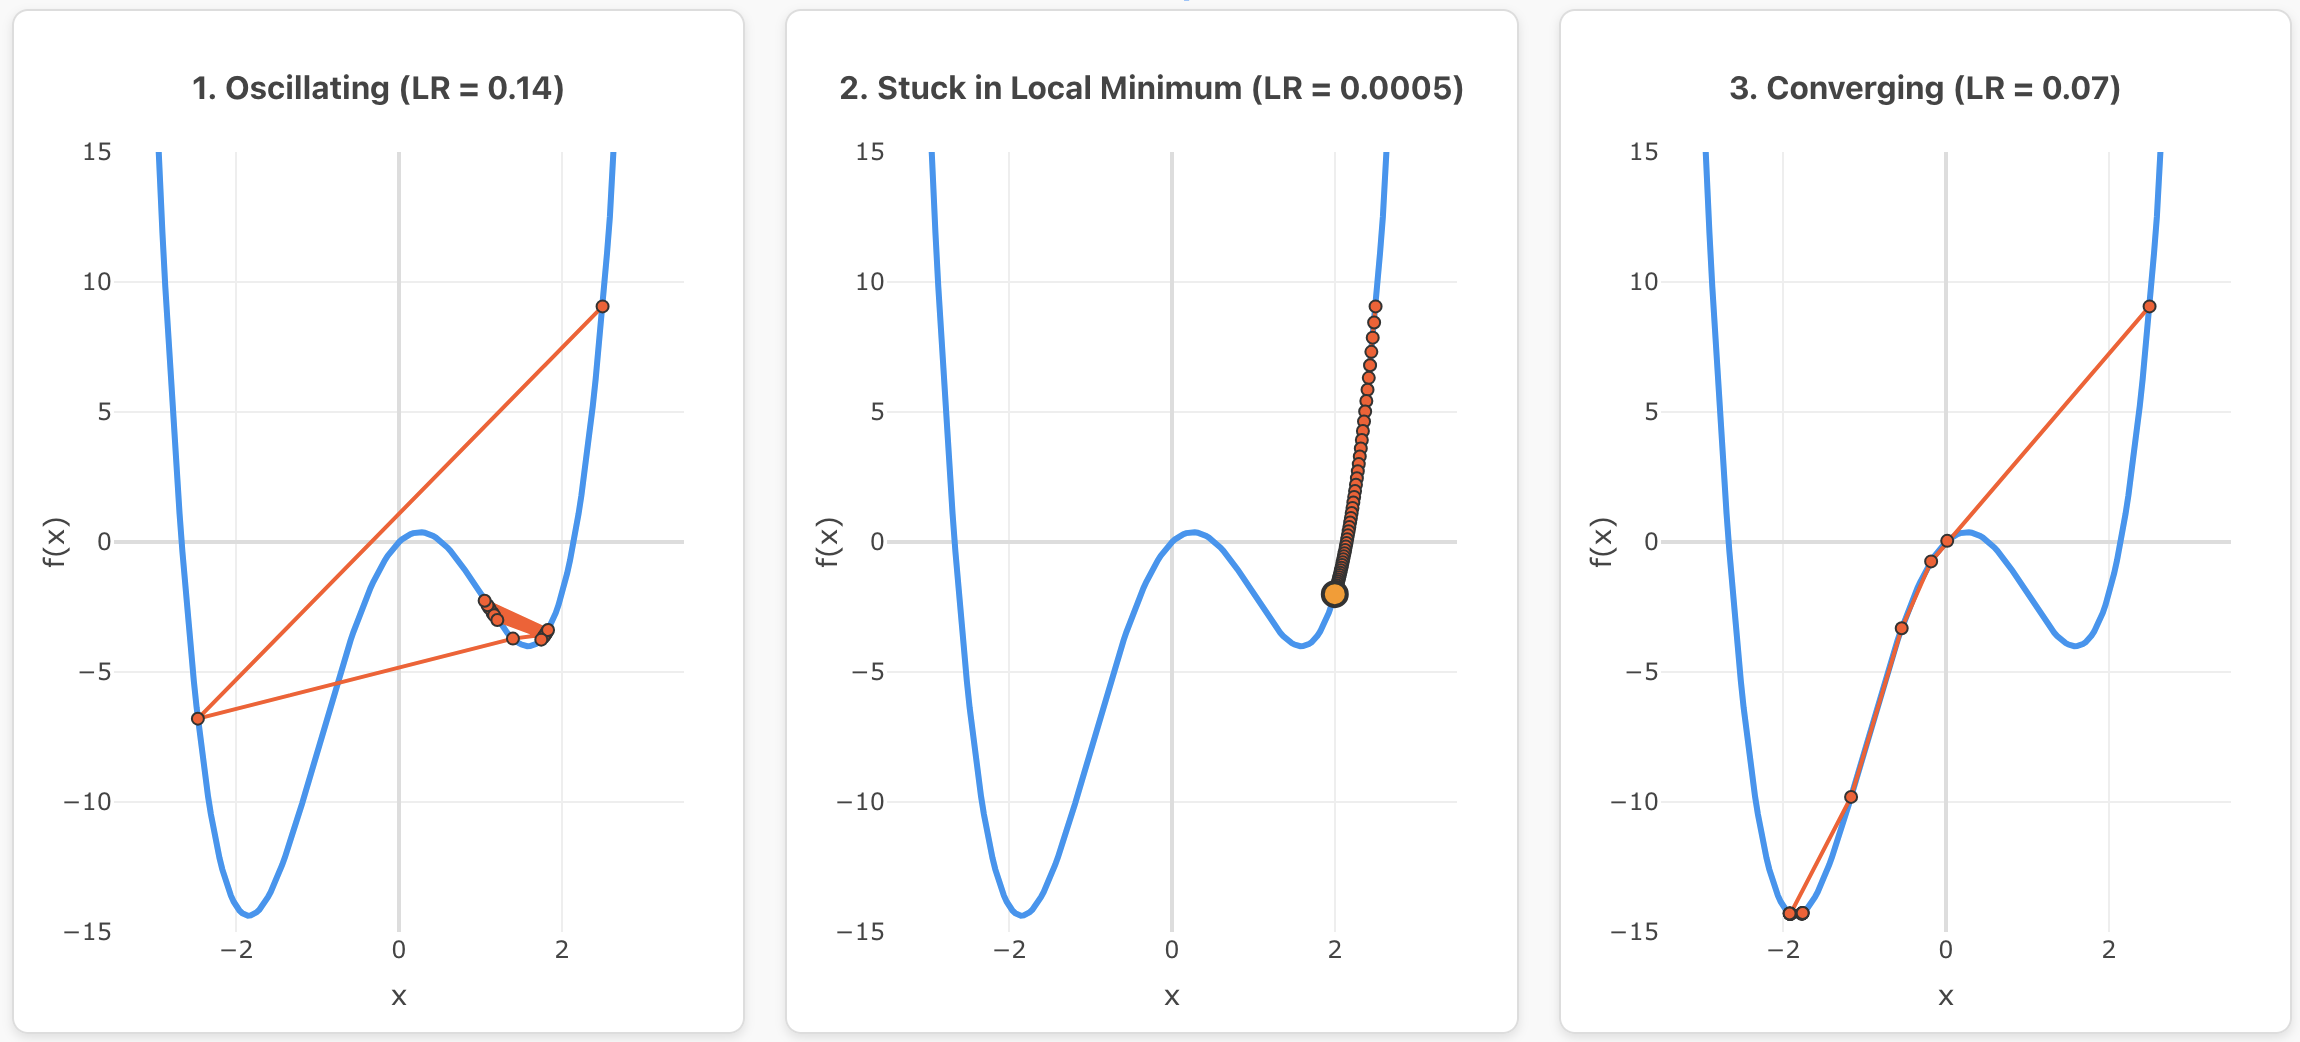
\includegraphics[width=0.6\textwidth]{figs/sgd.gif}
	\caption*{Gradient descent optimization}
\end{figure}

\end{frame}

%------------------------------------------------
\section{Experimental Results}

%------------------------------------------------
\begin{frame}
\frametitle{Width vs Approximation Quality}

\textbf{Hypothesis:} More neurons → better approximation

\textbf{Experiment:} Train networks with 5, 10, 20, 50 neurons

\begin{figure}[ht]
	\centering
	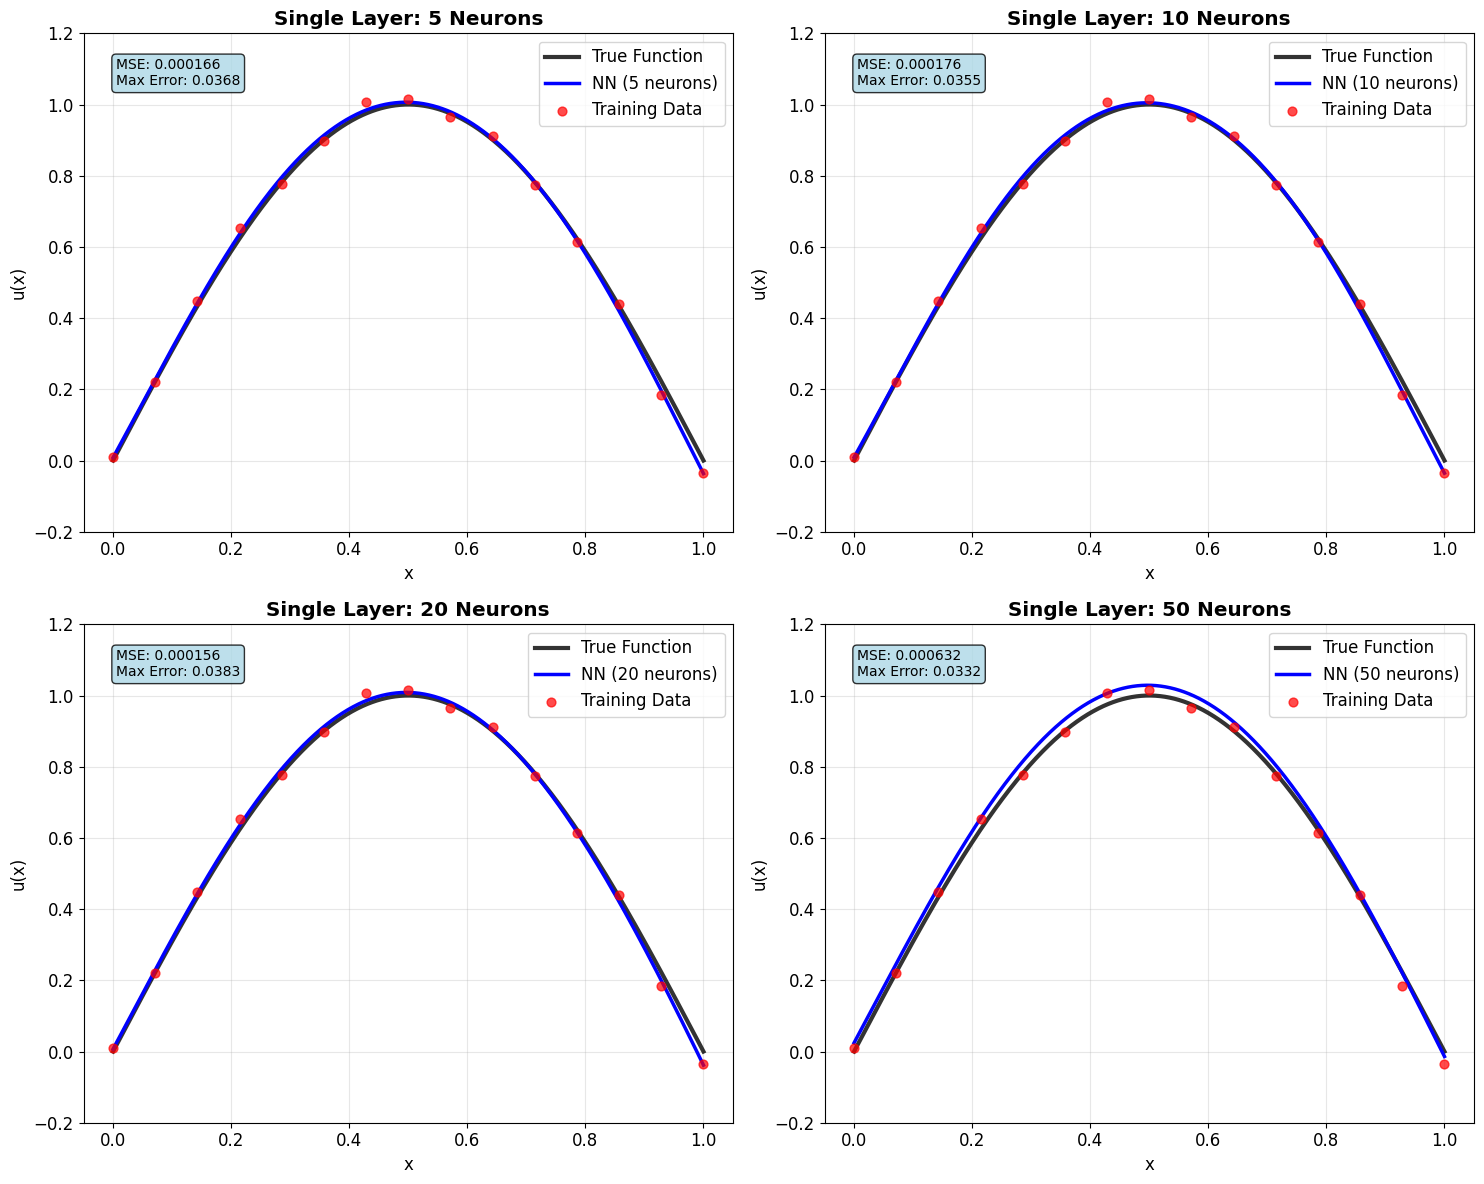
\includegraphics[width=0.9\textwidth]{figs/width-quality.png}
	\caption*{Approximation quality vs network width}
\end{figure}

\textbf{Results:} Clear improvement with increased width, validating Universal Approximation Theorem.

\end{frame}


%------------------------------------------------
\begin{frame}
\frametitle{Training/Validation}

\begin{figure}[ht]
	\centering
	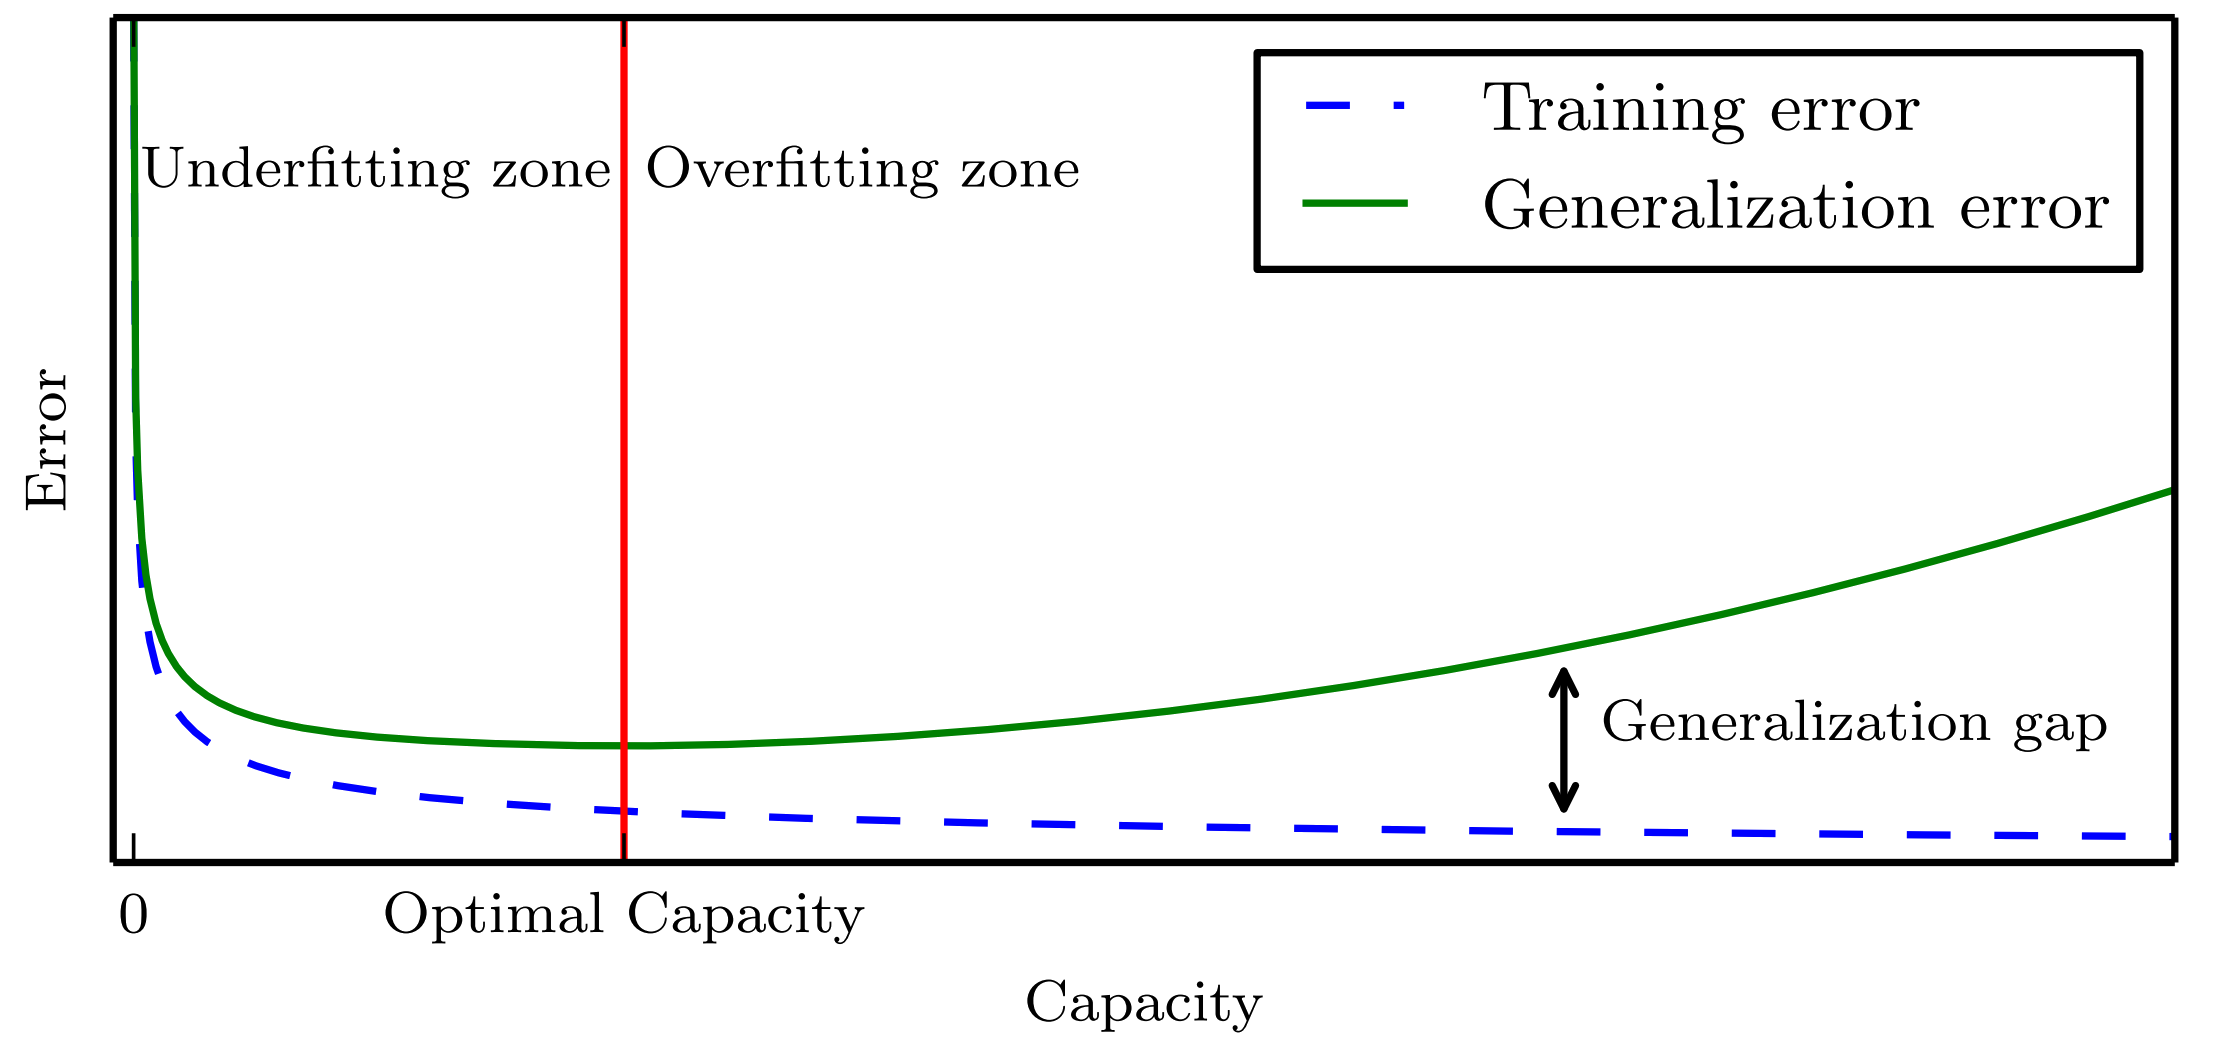
\includegraphics[width=0.9\textwidth]{figs/training-validation-fit.png}
	\caption*{Training and validation convergence}
\end{figure}

%------------------------------------------------
\begin{frame}
\frametitle{Training Convergence Analysis}

\begin{figure}[ht]
	\centering
	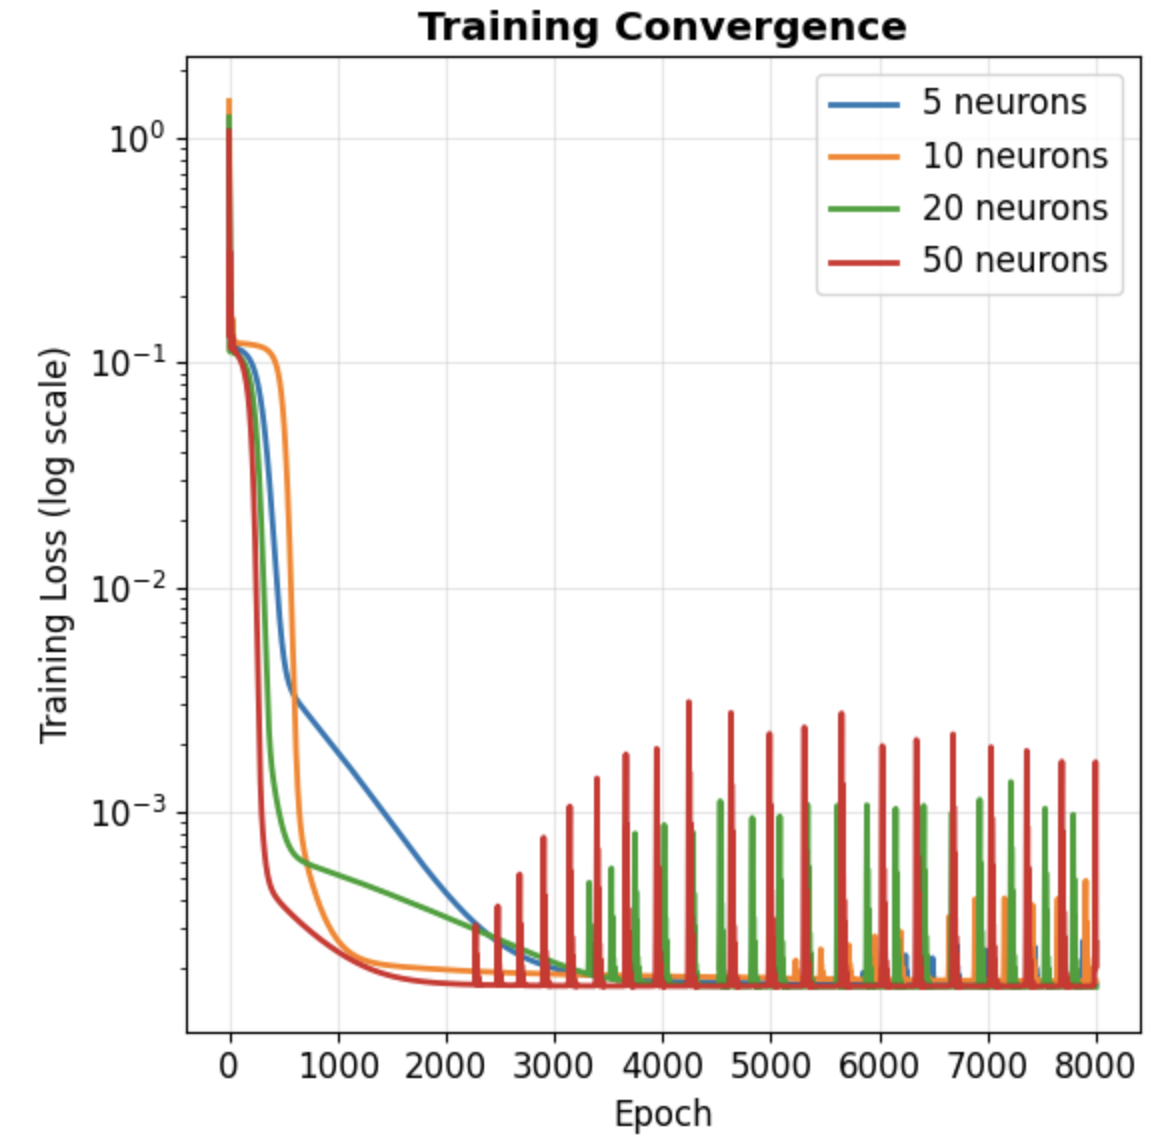
\includegraphics[width=0.9\textwidth]{figs/training-convergence.png}
	\caption*{Training convergence and final loss vs width}
\end{figure}

\textbf{Key Findings:}
\begin{itemize}
\item 50 neurons: $\sim$10x better than 5 neurons
\item Logarithmic improvement with width
\item Convergence rate similar across widths
\end{itemize}

\end{frame}

%------------------------------------------------
\begin{frame}
\frametitle{Overfitting and Model Capacity}

\textbf{Problem:} High-capacity networks can memorize training data.

\begin{figure}[ht]
	\centering
	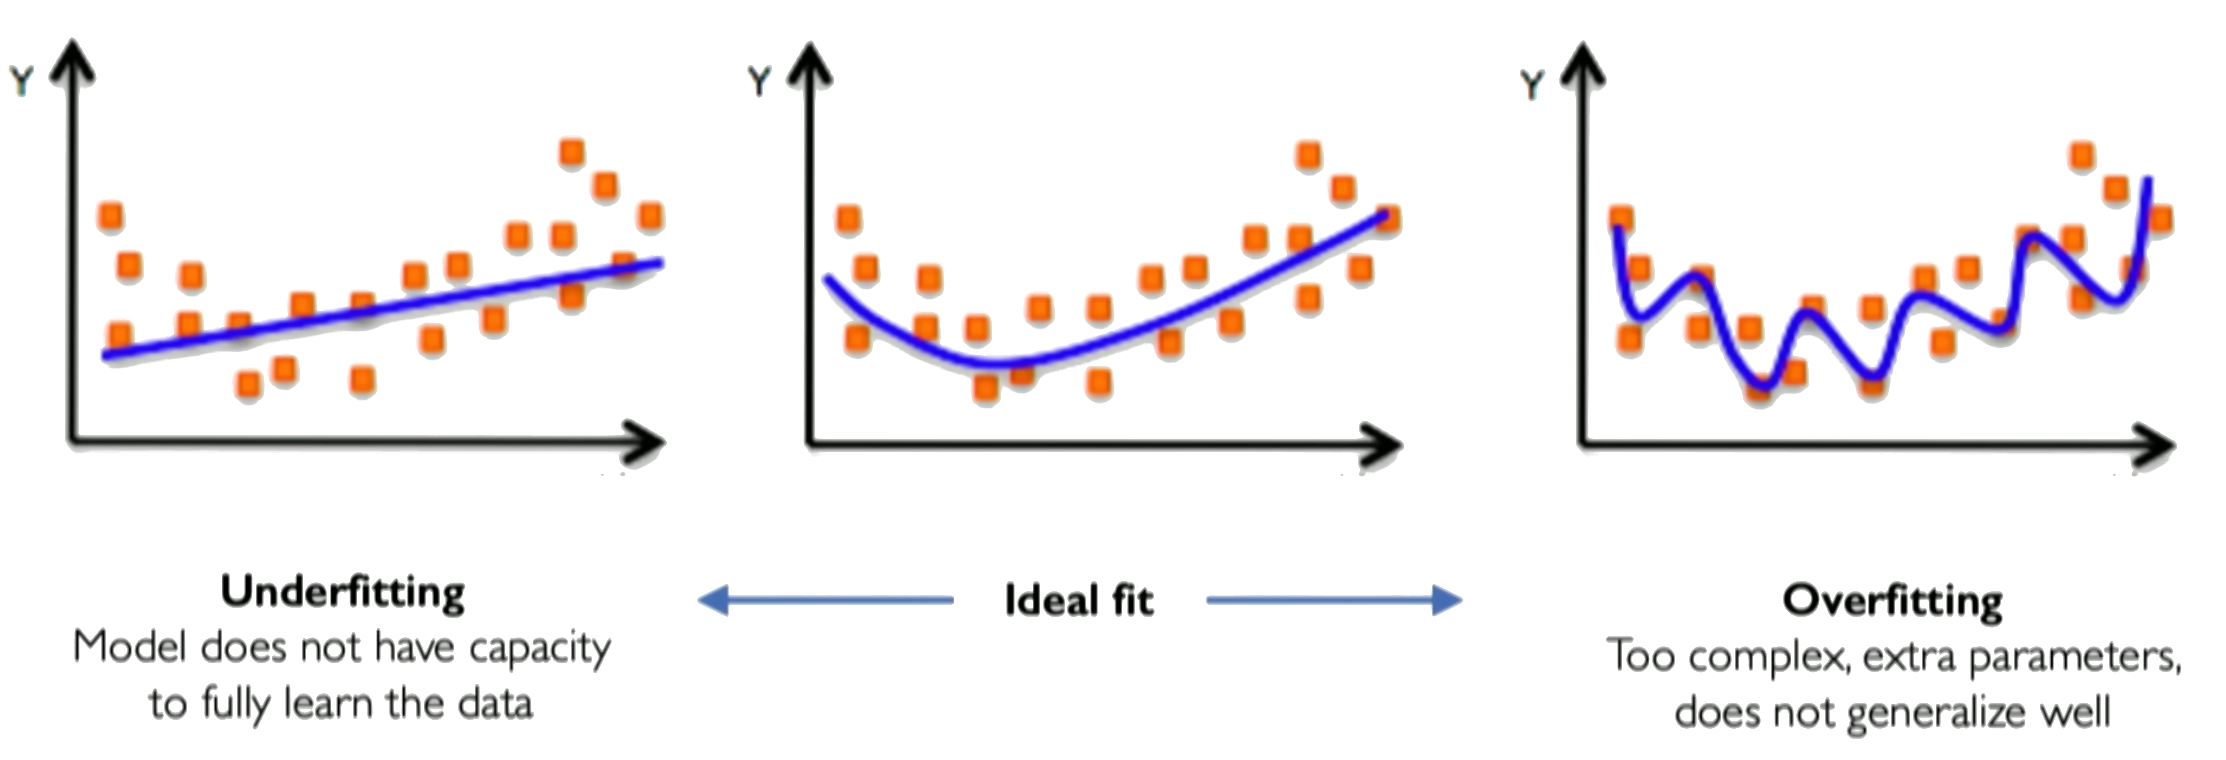
\includegraphics[width=0.7\textwidth]{figs/overfitting.png}
	\caption*{Under and overfitting illustration}
\end{figure}

\textbf{Detection:} Monitor validation loss during training.

\textbf{Solutions:} More data, regularization, early stopping, simpler architectures.

\end{frame}

%------------------------------------------------
\begin{frame}
\frametitle{Demonstrating Overfitting}

\begin{figure}[ht]
	\centering
	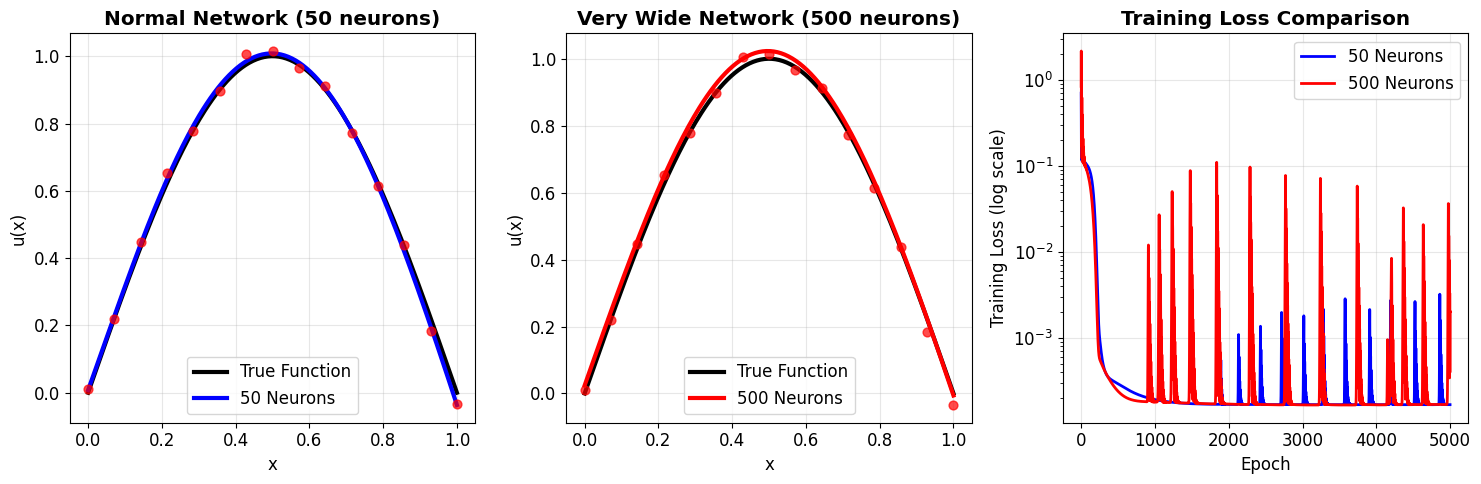
\includegraphics[width=0.9\textwidth]{figs/overfitting-demo.png}
	\caption*{Normal (50 neurons) vs very wide (500 neurons) network}
\end{figure}

\textbf{Observation:} Very wide networks may generalize worse despite lower training loss.

\end{frame}

%------------------------------------------------
\section{The Need for Depth}

%------------------------------------------------
\begin{frame}
\frametitle{The XOR Problem: Historical Crisis}

\textbf{XOR Truth Table:}
\begin{center}
\begin{tabular}{cc|c}
$x_1$ & $x_2$ & $y$ \\
\hline
0 & 0 & 0 \\
0 & 1 & 1 \\
1 & 0 & 1 \\
1 & 1 & 0 \\
\end{tabular}
\end{center}

\textbf{The Crisis:} No single line can separate these classes!

\begin{figure}[ht]
	\centering
	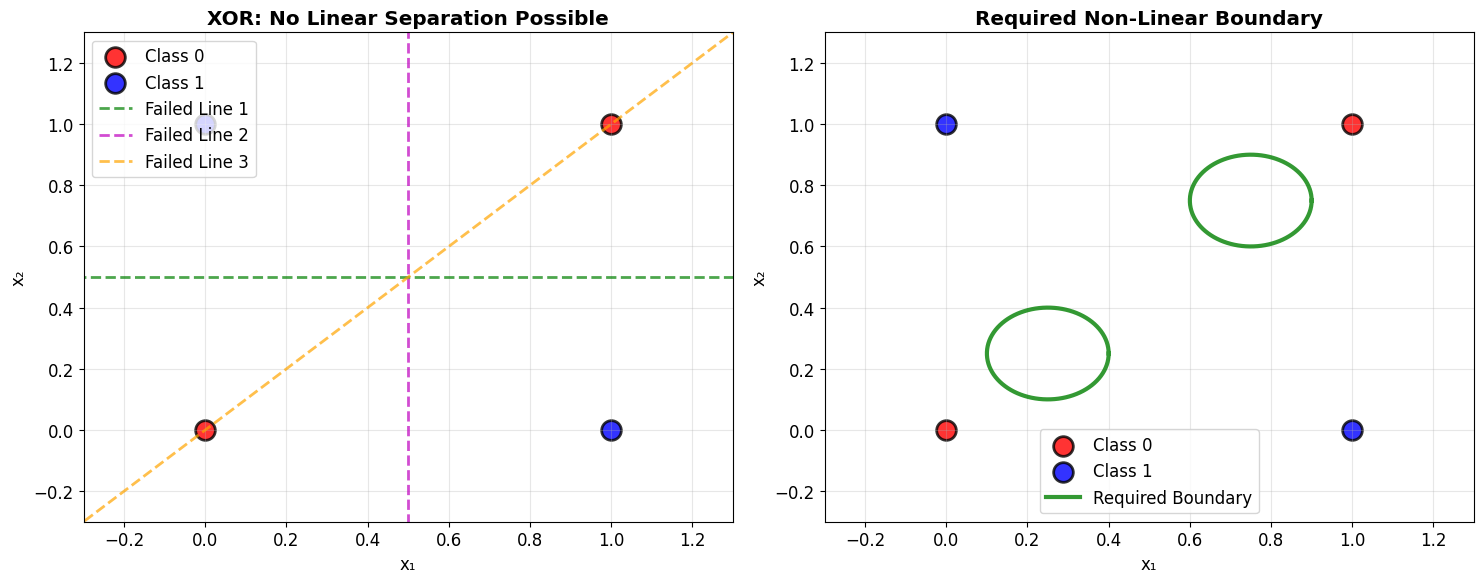
\includegraphics[width=0.8\textwidth]{figs/xor-problem.png}
	\caption*{XOR is not linearly separable}
\end{figure}

\end{frame}

%------------------------------------------------
\begin{frame}
\frametitle{True Single-Layer vs Multi-Layer}

\textbf{Critical Distinction:}
\begin{itemize}
\item \textbf{True Single-Layer:} Input $\to$ Output (NO hidden layers)
\item \textbf{Multi-Layer:} Input $\to$ Hidden $\to$ Output (1+ hidden layers)
\end{itemize}

\mode<beamer>{
\textbf{True Single-Layer (fails):}
\begin{equation*}
y = \sigma(w_1 x_1 + w_2 x_2 + b)
\end{equation*}

\textbf{Multi-Layer (succeeds):}
\begin{align*}
h_1 &= \sigma(w_{11} x_1 + w_{12} x_2 + b_1) \\
h_2 &= \sigma(w_{21} x_1 + w_{22} x_2 + b_2) \\
y &= \sigma(v_1 h_1 + v_2 h_2 + b_3)
\end{align*}
}
\mode<handout>{
\vspace{3cm}
}

\end{frame}

%------------------------------------------------
\begin{frame}
\frametitle{XOR Solution: Decision Boundaries}

\begin{figure}[ht]
	\centering
	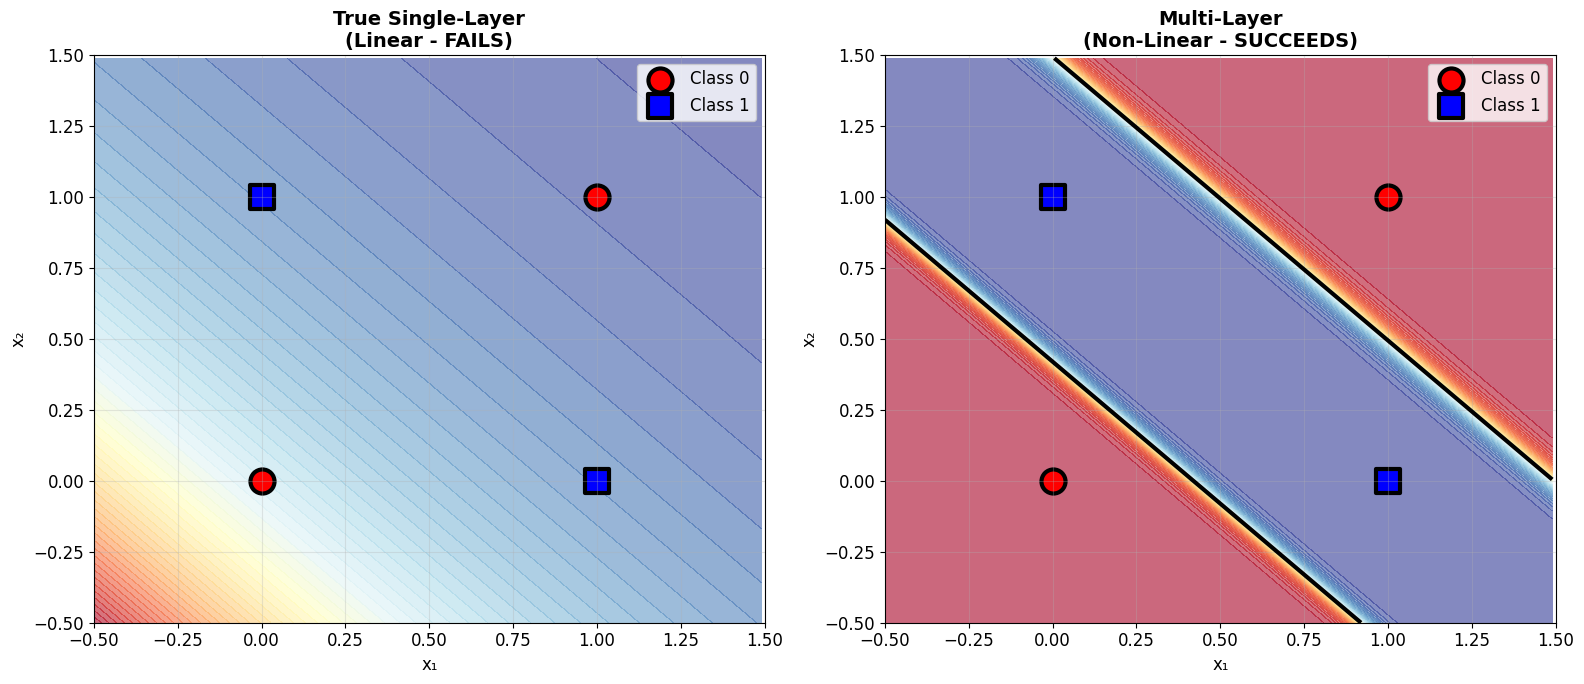
\includegraphics[width=0.9\textwidth]{figs/xor-decision-boundaries.png}
	\caption*{Linear (fails) vs Non-linear (succeeds) decision boundaries}
\end{figure}

\textbf{Key Insight:} Hidden layers enable curved boundaries through non-linear transformations.

\end{frame}

%------------------------------------------------
\begin{frame}
\frametitle{Mathematical Explanation}

\textbf{XOR Decomposition:}
\mode<beamer>{
\begin{align*}
h_1 &= \sigma(\text{weights}) \quad \text{(≈ OR gate)} \\
h_2 &= \sigma(\text{weights}) \quad \text{(≈ AND gate)} \\
y &= \sigma(v_1 h_1 + v_2 h_2 + b_3) \quad \text{(≈ OR AND NOT)}
\end{align*}

\textbf{Result:} XOR = (OR) AND (NOT AND) = compositional solution!
}
\mode<handout>{
\vspace{3cm}
}

\textbf{General Principle:} Complex functions = composition of simple functions.

\end{frame}

%------------------------------------------------
\begin{frame}
\frametitle{Beyond XOR: High-Frequency Functions}

\textbf{Test Case:} $f(x) = \sin(\pi x) + 0.3\sin(10\pi x)$

\begin{figure}[ht]
	\centering
	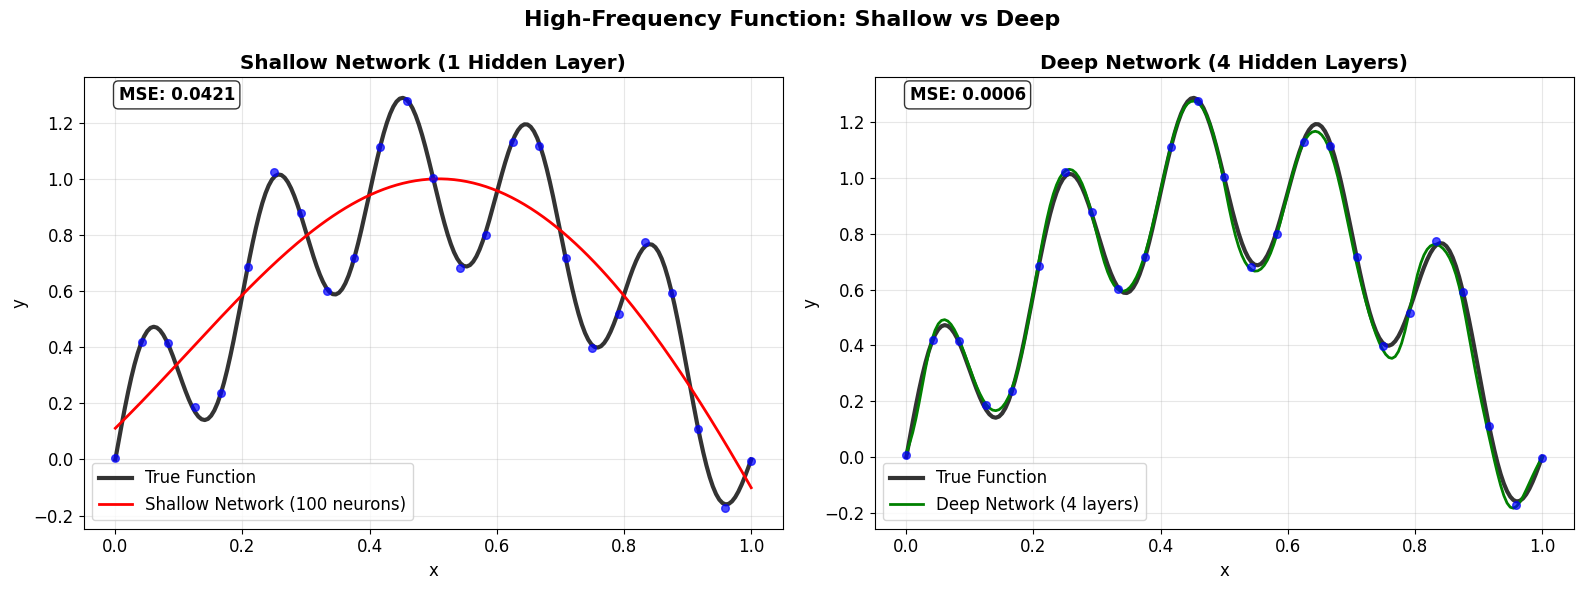
\includegraphics[width=0.9\textwidth]{figs/high-freq-comparison.png}
	\caption*{Shallow (100 neurons) vs Deep (4 layers, 25 each) networks}
\end{figure}

\textbf{Result:} Deep networks achieve better performance with fewer parameters.

\end{frame}

%------------------------------------------------
\begin{frame}
\frametitle{Historical Timeline: From Crisis to Revolution}

\begin{center}
\begin{tabular}{l|l|l}
\textbf{Year} & \textbf{Event} & \textbf{Impact} \\
\hline
1943 & McCulloch-Pitts neuron & Foundation laid \\
1957 & Rosenblatt's Perceptron & First learning success \\
\textbf{1969} & \textbf{Minsky \& Papert: XOR} & \textbf{Showed limits} \\
1970s-80s & "AI Winter" & Funding dried up \\
1986 & Backpropagation & Enabled multi-layer training \\
1989 & Universal Approximation & Theoretical foundation \\
2006+ & Deep Learning Revolution & Depth proves essential \\
\end{tabular}
\end{center}

\textbf{Lesson:} XOR taught us that depth is necessity, not luxury.

\end{frame}

%------------------------------------------------
\section{Why Depth Matters}

%------------------------------------------------
\begin{frame}
\frametitle{Four Key Insights on Depth}

\textbf{1. Representation Efficiency}
\begin{itemize}
\item Shallow: May need exponentially many neurons
\item Deep: Hierarchical composition is exponentially more efficient
\end{itemize}

\textbf{2. Feature Hierarchy}
\begin{itemize}
\item Layer 1: Simple features (edges, patterns)
\item Layer 2: Feature combinations (corners, textures)
\item Layer 3+: Complex abstractions (objects, concepts)
\end{itemize}

\textbf{3. Geometric Transformation}
\begin{itemize}
\item Each layer performs coordinate transformation
\item Deep networks "unfold" complex data manifolds
\end{itemize}

\textbf{4. Compositional Learning}
\begin{itemize}
\item Complex functions = composition of simple functions
\item Build complexity incrementally
\end{itemize}

\end{frame}

%------------------------------------------------
\begin{frame}
\frametitle{Summary and Conclusions}

\textbf{Key Takeaways:}
\begin{itemize}
\item Neural networks learn continuous functions from sparse data
\item Nonlinearity is essential for complex function approximation
\item Universal Approximation Theorem provides theoretical foundation
\item Width increases capacity but depth is more efficient
\item Historical XOR problem revealed importance of hidden layers
\item Deep networks enable hierarchical feature learning
\end{itemize}

\textbf{Applications:}
\begin{itemize}
\item Scientific computing and PDE solving
\item Function approximation and regression
\item Pattern recognition and classification
\item Physics-informed neural networks (PINNs)
\end{itemize}

\end{frame}

%------------------------------------------------
\begin{frame}
\frametitle{Questions?}

\centering
\Large Thank you!

\vspace{2cm}

\textbf{Contact:} \\
Krishna Kumar \\
\textit{krishnak@utexas.edu} \\
University of Texas at Austin

\end{frame}

\end{document}